\newif\ifshowsolutions
\showsolutionstrue
\documentclass{article}
\usepackage{listings}
\usepackage{amsmath}
%\usepackage{subfigure}
\usepackage{subfig}
\usepackage{amsthm}
\usepackage{amsmath}
\usepackage{amssymb}
\usepackage{graphicx}
\usepackage{mdwlist}
\usepackage[colorlinks=true]{hyperref}
\usepackage{geometry}
\usepackage{titlesec}
\geometry{margin=1in}
\geometry{headheight=2in}
\geometry{top=2in}
\usepackage{palatino}
\usepackage{mathrsfs}
\usepackage{fancyhdr}
\usepackage{paralist}
\usepackage{todonotes}
\setlength{\marginparwidth}{2.15cm}
\usepackage{tikz}
\usetikzlibrary{positioning,shapes,backgrounds}
\usepackage{float} % Place figures where you ACTUALLY want it
\usepackage{comment} % a hack to toggle sections
\usepackage{ifthen}
\usepackage{mdframed}
\usepackage{verbatim}
\usepackage[strings]{underscore}
\usepackage{listings}
\usepackage{bbm}
\rhead{}
\lhead{}

\renewcommand{\baselinestretch}{1.15}

% Shortcuts for commonly used operators
\newcommand{\E}{\mathbb{E}}
\newcommand{\Var}{\operatorname{Var}}
\newcommand{\Cov}{\operatorname{Cov}}
\newcommand{\Bias}{\operatorname{Bias}}
\DeclareMathOperator{\argmin}{arg\,min}
\DeclareMathOperator{\argmax}{arg\,max}

% do not number subsection and below
\setcounter{secnumdepth}{1}

% custom format subsection
\titleformat*{\subsection}{\large\bfseries}

% set up the \question shortcut
\newcounter{question}[section]
\newenvironment{question}[1][]
  {\refstepcounter{question}\par\addvspace{1em}\textbf{Question~\Alph{question}\!
    \ifthenelse{\equal{#1}{}}{}{ [#1 points]}: }}
    {\par\vspace{\baselineskip}}

\newcounter{subquestion}[question]
\newenvironment{subquestion}[1][]
  {\refstepcounter{subquestion}\par\medskip\textbf{\roman{subquestion}.\!
    \ifthenelse{\equal{#1}{}}{}{ [#1 points]:}} }
  {\par\addvspace{\baselineskip}}

\titlespacing\section{0pt}{12pt plus 2pt minus 2pt}{0pt plus 2pt minus 2pt}
\titlespacing\subsection{0pt}{12pt plus 4pt minus 2pt}{0pt plus 2pt minus 2pt}
\titlespacing\subsubsection{0pt}{12pt plus 4pt minus 2pt}{0pt plus 2pt minus 2pt}


\newenvironment{hint}[1][]
  {\begin{em}\textbf{Hint: }}{\end{em}}

\ifshowsolutions
  \newenvironment{solution}[1][]
    {\par\medskip \begin{mdframed}\textbf{Solution~\Alph{question}#1:} \begin{em}}
    {\end{em}\medskip\end{mdframed}\medskip}
  \newenvironment{subsolution}[1][]
    {\par\medskip \begin{mdframed}\textbf{Solution~\Alph{question}#1.\roman{subquestion}:} \begin{em}}
    {\end{em}\medskip\end{mdframed}\medskip}
\else
  \excludecomment{solution}
  \excludecomment{subsolution}
\fi

%%%%%%%%%%%%%%%%%%%%%%%%%%%%%%
% HEADER
%%%%%%%%%%%%%%%%%%%%%%%%%%%%%%

\chead{
  {\vbox{
      \vspace{2mm}
      \large
      Machine Learning \& Data Mining \hfill
      Caltech CS/CNS/EE 155 \hfill \\[1pt]
      Set 1\hfill
      January $4^{th}$, 2022 \\
    }
  }
}

\begin{document}
\pagestyle{fancy}



%%%%%%%%%%%%%%%%%%%%%%%%%%%%%%
% POLICIES
%%%%%%%%%%%%%%%%%%%%%%%%%%%%%%

\section*{Policies}
\begin{itemize}
	\item Due 9 PM PST, January $12^\text{th}$ on Gradescope. 
	\item You are free to collaborate on all of the problems, subject to the collaboration policy stated in the syllabus.
	\item If you have trouble with this homework, it may be an indication that you should drop the class.
	\item In this course, we will be using Google Colab for code submissions. You will need a Google account.
\end{itemize}

\section*{Submission Instructions}

\begin{itemize}
	\item Submit your report as a single .pdf file to Gradescope (entry code 7426YK), under "Set 1 Report". 
	\item In the report, \textbf{include any images generated by your code} along with your answers to the questions.
	\item Submit your code by \textbf{sharing a link in your report} to your Google Colab notebook for each problem (see naming instructions below). Make sure to set sharing permissions to at least "Anyone with the link can view". \textbf{Links that can not be run by TAs will not be counted as turned in.} Check your links in an incognito window before submitting to be sure. 
	\item For instructions specifically pertaining to the Gradescope submission process, see \url{https://www.gradescope.com/get_started#student-submission}.
	
\end{itemize}


\section*{Google Colab Instructions}

For each notebook, you need to save a copy to your drive.

\begin{enumerate}
	\item Open the github preview of the notebook, and click the icon to open the colab preview.
	\item On the colab preview, go to File $\rightarrow$ Save a copy in Drive.
	\item Edit your file name to “lastname_firstname_originaltitle”, e.g.”yue_yisong_3_notebook_part1.ipynb”
\end{enumerate}

%%%%%%%%%%%%%%%%%%%%%%%%%%%%%%
% PROBLEM 1
%%%%%%%%%%%%%%%%%%%%%%%%%%%%%%

\newpage
\section{Basics [16 Points]}
\materials{lecture 1}

Answer each of the following problems with 1-2 short sentences.

\begin{problem}[2]
  What is a hypothesis set?
\end{problem}
\begin{solution}
  The hypothesis set is the set that contains our hypothesis (which we hope approximates the target function).
\end{solution}

\begin{problem}[2]
  What is the hypothesis set of a linear model?
\end{problem}
\begin{solution}
  A hypothesis in the hypothesis set of a linear model has the general form of:
  \begin{equation}
    \mathbf{w}^T\mathbf{x}+b
  \end{equation}
\end{solution}

\begin{problem}[2]
  What is overfitting?
\end{problem}
\begin{solution}
  Overfitting is the situation where our test error is much greater than our training error, usually occuring when too many fitted parameters have been introduced to the model where these parameters now account for undesired aspects such as noise.
\end{solution}

\begin{problem}[2]
  What are two ways to prevent overfitting?
\end{problem}
\begin{solution}
  1. Splitting our training data into a training set and validation set, performing cross-validation to fit the model.
  2. Use fitting strategies such as ridge, lasso and elastic net regression which constraint the fitted parameters to avoid overfitting.
\end{solution}

\begin{problem}[2]
  What are training data and test data, and how are they used differently? Why should you never change your model based on information from test data?
\end{problem}
\begin{solution}
  Training data is used to fit the model whilst testing data is used to evaluate the performance of the model. As a result, for a testing set to serve is purpose properly, it cannot be involved in the training of the model, despite the fact it may improve the performance (although, as a result of using the testing data, we will not be able to properly evaluate this).
\end{solution}

\begin{problem}[2]
  What are the two assumptions we make about how our dataset is sampled?
\end{problem}
\begin{solution}
  1. It is assumed that the inputs of this dataset are sampled independently of the `true' distribution. 
  2. It is assumed that the outputs of this dataset accurately represent the output space (e.g. if we're sampling COVID test results, we would expect our ouputs to contain positive, negative and inconclusive outputs)
\end{solution}

\begin{problem}[2]
  Consider the machine learning problem of deciding whether or not an email is spam. What could $X$, the input space, be? What could $Y$, the output space, be?
\end{problem}
\begin{solution}
  X could be the the `bag of words' used in the email, the sender's email address, the email title \textit{etc.}.
  Y could be spam or not spam [0 and 1 binary values].
\end{solution}

\begin{problem}[2]
  What is the $k$-fold cross-validation procedure?
\end{problem}
\begin{solution}
  This involves first splitting our training set into $k$ manifolds. In a given iteration, we select $k-1$ manifolds to train our data on and the remaining manifold to evaluate the model performance. This is repeated $k$ times with different manifolds being used to evaluate the model each time. 
\end{solution}



%%%%%%%%%%%%%%%%%%%%%%%%%%%%%%
% PROBLEM 2
%%%%%%%%%%%%%%%%%%%%%%%%%%%%%%

\newpage
\section{Bias-Variance Tradeoff [34 Points]}
\materials{lecture 1}

\begin{problem}[5]
  Derive the bias-variance decomposition for the squared error loss function. That is, show that for a model $f_S$ trained on a dataset $S$ to predict a target $y(x)$ for each $x$,
  \begin{align*}
    \E_S \left[E_\text{out}\left(f_S\right)\right] = \E_x[\Bias(x) + \Var(x)]
  \end{align*}
  given the following definitions:
  \begin{align*}
    F(x) &= \E_S\left[f_S(x) \right] \\
    E_\text{out}(f_S) &= \E_x\left[\left(f_S(x) - y(x)\right)^2\right] \\
    \Bias(x) &= (F(x) - y(x))^2 \\
    \Var(x) &= \E_S\left[(f_S(x)-F(x))^2\right]
  \end{align*}
\end{problem}

\begin{solution}
  \begin{equation}
  \E_S[E_\text{out}(f_S)] = \E_S[\E_x\left[\left(f_S(x) - y(x)\right)^2\right]]
  \end{equation}
  \begin{equation}
    \E_S[E_\text{out}(f_S)] = \E_S\left[\E_x\left[\left(f_S(x)-F(x) +F(x) - y(x)\right)^2\right]\right]
  \end{equation}
  \begin{equation}
    \E_S[E_\text{out}(f_S)] = \E_S\left[\E_x\left[\left(f_S(x)-F(x)\right)^2 +\left(F(x) - y(x)\right)^2+2\left(f_S(x)-F(x)\right)\left(F(x) - y(x)\right)\right]\right]
  \end{equation}
  \begin{equation}
    \E_S[E_\text{out}(f_S)] = \E_x\left[\E_S\left[\left(f_S(x)-F(x)\right)^2\right] +\E_S\left[\left(F(x) - y(x)\right)^2\right]+2\E_S\left[\left(f_S(x)-F(x)\right)\left(F(x) - y(x)\right)\right]\right]
  \end{equation}
  \begin{equation}
    \E_S[E_\text{out}(f_S)] = \E_x\left[\E_S\left[\left(f_S(x)-F(x)\right)^2\right] +\E_S\left[\left(F(x) - y(x)\right)^2\right]\right]
  \end{equation}
  \begin{equation}
    \E_S[E_\text{out}(f_S)] = \E_x\left[\E_S\left[\left(f_S(x)-F(x)\right)^2\right] +\left(F(x) - y(x)\right)^2\right]
  \end{equation}
  \begin{equation}
    \E_S \left[E_\text{out}\left(f_S\right)\right] = \E_x[\Bias(x) + \Var(x)]
  \end{equation}
\end{solution}

In the following problems you will explore the bias-variance tradeoff by producing learning curves for polynomial regression models.

A \emph{learning curve} for a model is a plot showing both the training error and the cross-validation error as a function of the number of points in the training set. These plots provide valuable information regarding the bias and variance of a model and can help determine whether a model is over-- or under--fitting.

\emph{Polynomial regression} is a type of regression that models the target $y$ as a degree--$d$ polynomial function of the input $x$. (The modeler chooses $d$.)  You don't need to know how it works for this problem, just know that it produces a polynomial that attempts to fit the data.

\begin{problem}[14]
    Use the provided \texttt{2_notebook.ipynb} Jupyter notebook to enter your code for this question. This notebook contains examples of using NumPy's polyfit and polyval methods, and scikit-learn's KFold method; you may find it helpful to read through and run this example code prior to continuing with this problem. Additionally, you may find it helpful to look at the documentation for scikit-learn's learning_curve method for some guidance.

The dataset \texttt{bv_data.csv} is provided and has a header denoting which columns correspond to which values. Using this dataset, plot learning curves for 1st--, 2nd--, 6th--, and 12th--degree polynomial regression (4 separate plots) by following these steps for each degree $d \in \{1, 2, 6, 12\}$:

  \begin{enumerate}
    \item For each $N \in \{20, 25, 30, 35, \cdots, 100\}$:
    \begin{enumerate}[i.]
      \item Perform 5-fold cross-validation on the first $N$ points in the dataset (setting aside the other points), computing the both the training and validation error for each fold. 
      \begin{itemize}
        \item Use the mean squared error loss as the error function.
        \item Use NumPy's polyfit method to perform the degree--$d$ polynomial regression and NumPy's polyval method to help compute the errors.  (See the example code and \href{https://docs.scipy.org/doc/NumPy/reference/routines.polynomials.poly1d.html}{NumPy documentation} for details.)
        \item When partitioning your data into folds, although in practice you should randomize your partitions, for the purposes of this set, simply divide the data into $K$ contiguous blocks.
      \end{itemize}
      \item Compute the average of the training and validation errors from the 5 folds.
    \end{enumerate}
    \item Create a learning curve by plotting both the average training and validation error as functions of $N$. \textit{Hint: Have same y-axis scale for all degrees $d$.}
  \end{enumerate}

\end{problem}
\begin{solution}
  Link: \url{https://colab.research.google.com/drive/18sjMP0ADNXw8WxW4mZiMroxFu20poX9e?usp=sharing}
  \begin{figure}[H]
    \subfloat[]{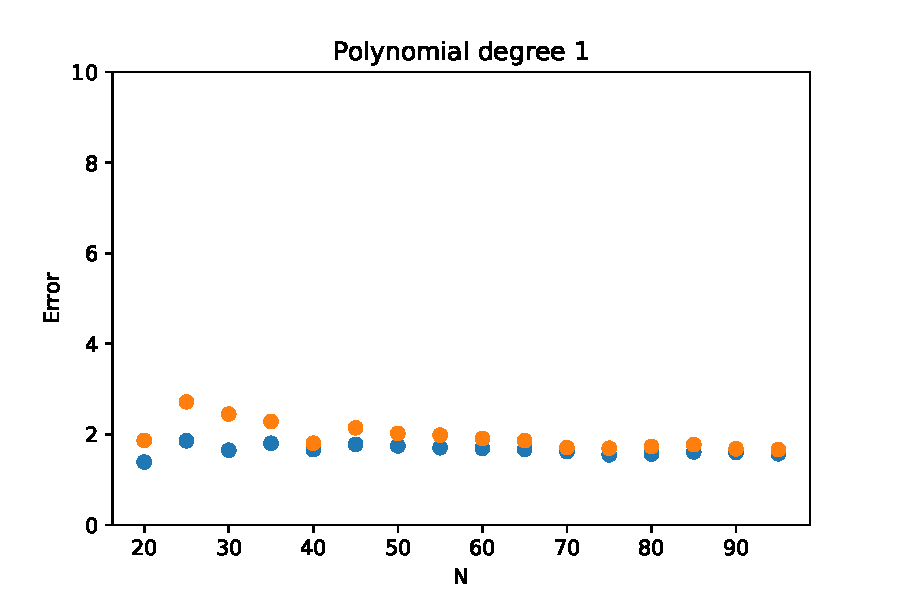
\includegraphics[width=0.49\textwidth]{poly_1.pdf}}
    \subfloat[]{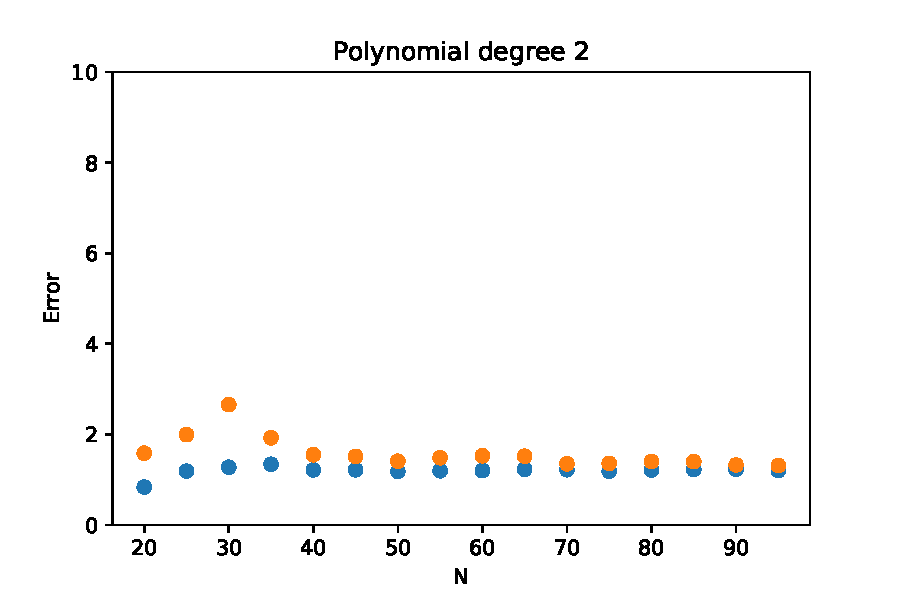
\includegraphics[width=0.49\textwidth]{poly_2.pdf}}\\
    \subfloat[]{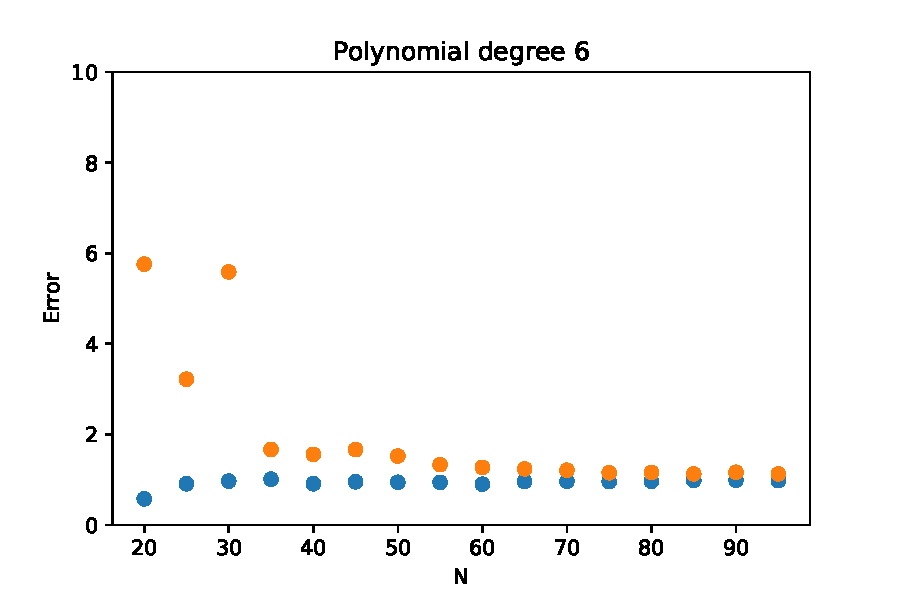
\includegraphics[width=0.49\textwidth]{poly_6.pdf}}
    \subfloat[]{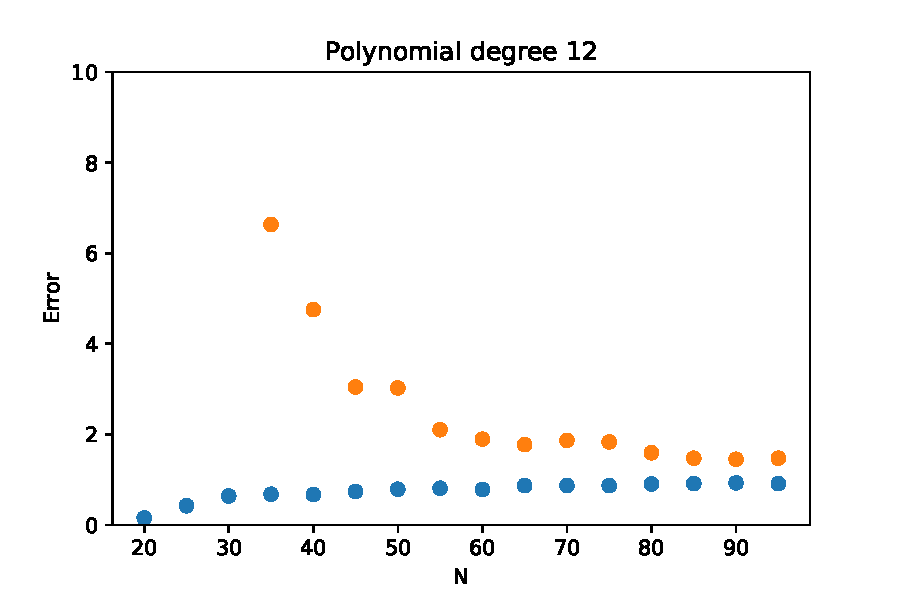
\includegraphics[width=0.49\textwidth]{poly_12.pdf}}
  \end{figure}
  \end{solution}

\begin{problem}[3]
  Based on the learning curves, which polynomial regression model (i.e. which degree polynomial) has the highest bias? How can you tell?
\end{problem}
\begin{solution}
 The model with the highest bias is the linear model as its training error is largest for all $N$. This is to be expected as it is most likely that the dataset contains certain complexities that cannot be captured using a linear model.
\end{solution}

\begin{problem}[3]
  Which model has the highest variance? How can you tell?
\end{problem}
\begin{solution}
  The 12-$th$ order polynomial has the largest variance as it has the largest difference in error between the validation and training set. This is another example of overfitting where the additional parameters are accounting for the unphysical noise in the data and not capturing the actual trend, resulting in the higher validation error.
\end{solution}

\begin{problem}[3]
  What does the learning curve of the quadratic model tell you about how much the model will improve if we had additional training points?
\end{problem}
\begin{solution}
 As we increase $N$, the validation error appears to approach the training error. The training error plateaux early on at low $N$ whilst the validation error asymtotically approach the training error. This implies that the quadratic model may generalise well.
\end{solution}

\begin{problem}[3]
  Why is training error generally lower than validation error?
\end{problem}
\begin{solution}
  This is to be expected as the fitted model was designed to minimise the error in the training set. If the validation set is selected properly, then, in the ideal scenario, our fitted model will be perfect and the errors will be the same. However, more likely than not, there will be noise in both datasets and the validation model may contain behaviours not captured by the training set, increasing the validation error. 
\end{solution}

\begin{problem}[3]
  Based on the learning curves, which model would you expect to perform best on some unseen data drawn from the same distribution as the training data, and why?
\end{problem}
\begin{solution}
  For $N=100$ data points, the 6-$th$ degree polynomial has the lowest validation error. Although the validation and training errors aren't as similar as they are compared to the quadratic model, this lower validation error does imply this model should perform better on unseen data.
\end{solution}




%%%%%%%%%%%%%%%%%%%%%%%%%%%%%%
% PROBLEM 3
%%%%%%%%%%%%%%%%%%%%%%%%%%%%%%

\newpage
\section{Stochastic Gradient Descent [36 Points]}
\materials{lecture 2}

Stochastic gradient descent (SGD) is an important optimization method in machine learning, used everywhere from logistic regression to training neural networks. In this problem, you will be asked to first implement SGD for linear regression using the squared loss function. Then, you will analyze how several parameters affect the learning process.

Linear regression learns a model of the form:
\begin{align*}
  f(x_1, x_2, \cdots, x_d) = \left(\sum_{i=1}^d w_i x_i\right) + b
\end{align*}

% problem A tests the students understanding of matrix representations and serves are a reminder that the bias term is still there.
\begin{problem}[2]
  We can make our algebra and coding simpler by writing $f(x_1, x_2, \cdots, x_d) = \mathbf{w}^T\mathbf{x}$ for vectors $\mathbf{w}$ and $\mathbf{x}$.  But at first glance, this formulation seems to be missing the bias term $b$ from the equation above.  How should we define $\mathbf{x}$ and $\mathbf{w}$ such that the model includes the bias term?
\end{problem}
\begin{hint}
  Include an additional element in $\mathbf{w}$ and $\mathbf{x}$.
\end{hint}
\begin{solution}
  We add a new element to the $\mathbf{w}$ vector: $w_0=b$ and add a new element to the $\mathbf{x}$ vector: $x_0=1$. All other elements $1,\hdots,d$ remain the same.
\end{solution}

Linear regression learns a model by minimizing the squared loss function $L$, which is the sum across all training data $\{(\mathbf{x}_1, y_1),\cdots,(\mathbf{x}_N, y_N)\}$ of the squared difference between actual and predicted output values:
\[L(f) = \sum_{i=1}^N (y_i - \mathbf{w}^T\mathbf{x}_i)^2\]

\begin{problem}[2]
  SGD uses the gradient of the loss function to make incremental adjustments to the weight vector $\mathbf{w}$. Derive the gradient of the squared loss function with respect to $\mathbf{w}$ for linear regression.
\end{problem}
\begin{solution}
  \begin{equation}
    \nabla_\mathbf{w}L(f) = \nabla_\mathbf{w}\left[\sum_{i=1}^N y_i^2 - 2y_i\mathbf{w}^T\mathbf{x}_i+(\mathbf{w}^T\mathbf{x}_i)^2\right]
  \end{equation}
  \begin{equation}
    \nabla_\mathbf{w}L(f) = - 2\sum_{i=1}^N (y_i-\mathbf{w}^T\mathbf{x}_i)\mathbf{x}_i
  \end{equation}
\end{solution}

The following few problems ask you to work with the first of two provided Jupyter notebooks for this problem, \texttt{3_notebook_part1.ipynb}, which includes tools for gradient descent visualization. This notebook utilizes the files \texttt{sgd_helper.py} and \texttt{multiopt.mp4}, but you should not need to modify either of these files. 

For your implementation of problems C-E, \textbf{do not} consider the bias term.

\begin{problem}[8]
  Implement the \texttt{loss}, \texttt{gradient}, and \texttt{SGD} functions, defined in the notebook, to perform SGD, using the guidelines below:

  \begin{itemize}
    \item Use a squared loss function.
    \item Terminate the SGD process after a specified number of epochs, where each epoch performs one SGD iteration for each point in the dataset.
    \item It is recommended, but not required, that you shuffle the order of the points before each epoch such that you go through the points in a random order. You can use \texttt{numpy.random.permutation}.
    \item Measure the loss after each epoch. Your \texttt{SGD} function should output a vector with the loss after each epoch, and a matrix of the weights after each epoch (one row per epoch). Note that the weights from all epochs are stored in order to run subsequent visualization code to illustrate SGD.
  \end{itemize}
\end{problem}
\begin{solution}
See code. %This does not need to be changed.
\end{solution}

\begin{problem}[2]
  Run the visualization code in the notebook corresponding to problem D. How does the convergence behavior of SGD change as the starting point varies? How does this differ between datasets 1 and 2? Please answer in 2-3 sentences.
\end{problem}
\begin{solution}
  Link: \url{https://colab.research.google.com/drive/110b7vOryXQQPvu6pNwGutkXwQU6ucG0h?usp=sharing}
 It appears that the starting point does not have a significant impact on the convergence of SGD as, regardless of the starting point, the solutions converge to the same point at around the same time, with the furtherest point taking marginally longer than the rest. Similarly, it seems the dataset itself doesn't affect the convergence rate of each starting point relative to the other. The reason for this could be due to the fact that the loss function is nice and convex, not having any significant changes in convexity or any local minima.
\end{solution}

\begin{problem}[6]
  Run the visualization code in the notebook corresponding to problem E. One of the cells---titled "Plotting SGD Convergence"---must be filled in as follows. Perform SGD on dataset 1 for each of the learning rates $\eta \in$ \{1e-6, 5e-6, 1e-5, 3e-5, 1e-4\}. On a single plot, show the training error vs. number of epochs trained for each of these values of $\eta$. What happens as $\eta$ changes?
\end{problem}

\begin{solution}
 \begin{figure}[H]
  \subfloat[]{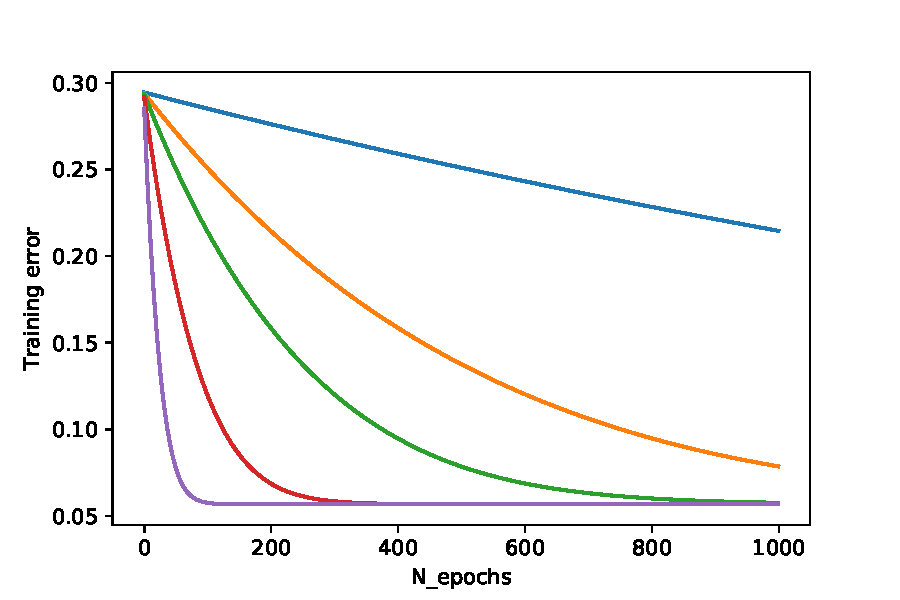
\includegraphics[width=0.7\textwidth]{err_train_SGD.pdf}}
 \end{figure}
 As we can see, as we increase $\eta$, the rate of convergence increases, where our largest value of $\eta$ plateaux at around 100 epochs. However, that isn't to say increasing $\eta$ will always improve the rate of convergence. If $\eta$ is too large, we may over-shoot the true minima, resulting in the algorithm oscilating around the true solution (or even diverging in the worst-case scenario).
\end{solution}


The following problems consider SGD with the larger, higher-dimensional dataset, \texttt{sgd_data.csv}. The file has a header denoting which columns correspond to which values. For these problems, use the Jupyter notebook \texttt{3_notebook_part2.ipynb}.

For your implementation of problems F-H, \textbf{do} consider the bias term using your answer to problem A.

\begin{problem}[6]
  Use your SGD code with the given dataset, and report your final weights. Follow the guidelines below for your implementation:

  \begin{itemize}
    \item Use $\eta = e^{-15}$ as the step size.  
    \item Use $\mathbf{w} = [0.001, 0.001, 0.001, 0.001]$ as the initial weight vector and $b = 0.001$ as the initial bias.
    \item Use at least 800 epochs.
    \item You should incorporate the bias term in your implementation of SGD and do so in the vector style of problem A.
    \item Note that for these problems, it is no longer necessary for the \texttt{SGD} function to store the weights after all epochs; you may change your code to only return the final weights.
  \end{itemize}
  %$\epsilon$ here is a measure of how much change in error there is compared to the initial error in the epoch. Calculate the change in error every epoch and compare it to the change in error from the first epoch. If new change/initial change is less than $\epsilon$, stop the training. $\eta$ is the factor by which you multiply the gradient in each step of the descent, and $\mathbf{w}$ is the initial weight vector.
\end{problem}
\begin{solution}
  The following weights were obtained:
  
  $\mathbf{w}=$[ -5.94229011   3.94369494 -11.72402388   8.78549375  -0.22720591]
\end{solution}

\begin{problem}[2]
  Perform SGD as in the previous problem for each learning rate $\eta$ in \[\{e^{-10}, e^{-11}, e^{-12}, e^{-13}, e^{-14}, e^{-15}\},\] and calculate the training error at the beginning of each epoch during training.  On a single plot, show training error vs. number of epochs trained for each of these values of $\eta$. Explain what is happening.
\end{problem}
\begin{solution}
  \begin{figure}[H]
    \subfloat[]{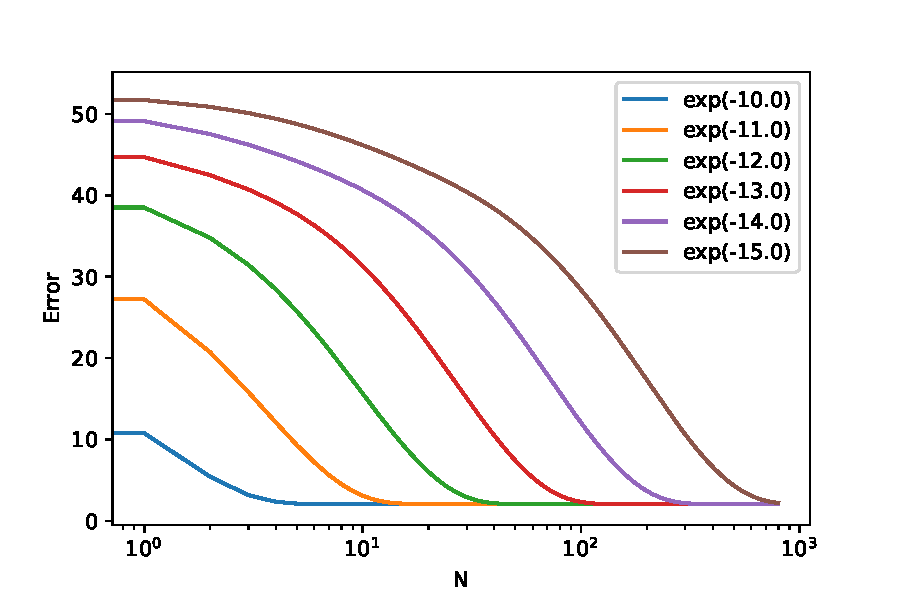
\includegraphics[width=0.7\textwidth]{SGD_3G.pdf}}
   \end{figure}
   As we can see above, as we increase the learning rate, we converge to the optimal weights faster. As explained previously, we don't expect this trend to continue forever; eventually $\eta$ will get too large that we will just oscilate around the optimal solution.
\end{solution}


\begin{problem}[2]
  The closed form solution for linear regression with least squares is \[\mathbf{w} = \left(\sum_{i=1}^N \mathbf{x_i}\mathbf{x_i}^T\right)^{-1}\left(\sum_{i=1}^N \mathbf{x_i}y_i\right).\]  Compute this analytical solution.  Does the result match up with what you got from SGD?
\end{problem}
\begin{solution}
  Link: \url{https://colab.research.google.com/drive/18-vtFm-zo8FgV1DoXhesaWBiGQ-WVJgM?usp=sharing}
 The weights obtained using least squares is:

 $\mathbf{w}=$[ -5.99157048   4.01509955 -11.93325972   8.99061096  -0.31644251]

 This is indeed very close to the solution obtained using SGD (approximately a 7\% error).
\end{solution}

Answer the remaining questions in 1-2 short sentences.

\begin{problem}[2]
  Is there any reason to use SGD when a closed form solution exists?
\end{problem}
\begin{solution}
  Least square regression can only apply to problems whose objective function is squared distance between the estimates and true values; SGD can be applied to any objective function as long as it is differentiable. This increases the range of problems it can be applied to.
\end{solution}

\begin{problem}[2]
  Based on the SGD convergence plots that you generated earlier, describe a stopping condition that is more sophisticated than a pre-defined number of epochs.
\end{problem}
\begin{solution}
  We could specify a value of the loss function or step size (relative or absolute) after which the SGD algorithm can terminate (e.g. if the loss function or relative step size is less than $10^{-8}$). Similarly, if the validation error increases, regardless of our learning rate, we can terminate the SGD algorithm.
\end{solution}

\begin{problem}[2]
How does the convergence behavior of the weight vector differ between the perceptron and SGD algorithms?
\end{problem}
\begin{solution}
  In the SGD algorithm, the weight vector eventually converges with smaller and smaller step sizes, given the length of the gradient becomes smaller as we approach the optimum. For the PLA algorithm, the step size scales with the length of our data points $\mathbf{x}$, as such, the size of the step remains largerly the same throughout the algorithm, even when approaching the optimum solution.
\end{solution}




%%%%%%%%%%%%%%%%%%%%%%%%%%%%%%
% PROBLEM 4
%%%%%%%%%%%%%%%%%%%%%%%%%%%%%%

\newpage
\section{The Perceptron [14 Points]}
\materials{lecture 2}

The perceptron is a simple linear model used for binary classification. For an input vector $\mathbf{x} \in \mathbb{R}^d$, weights $\mathbf{w} \in \mathbb{R}^d$, and bias $b \in \mathbb{R}$, a perceptron $f: \mathbb{R}^d \rightarrow \{-1,1\}$ takes the form
\begin{align*}
  f(\mathbf{x}) = \operatorname{sign}\left(\left(\sum_{i=1}^d w_i x_i\right) + b \right)
\end{align*}

The weights and bias of a perceptron can be thought of as defining a hyperplane that divides $\mathbb{R}^d$ such that each side represents an output class. For example, for a two dimensional dataset, a perceptron could be drawn as a line that separates all points of class $+1$ from all points of class $-1$.

The PLA (or the Perceptron Learning Algorithm) is a simple method of training a perceptron. First, an initial guess is made for the weight vector $\mathbf{w}$. Then, one misclassified point is chosen arbitrarily and the $\mathbf{w}$ vector is updated by
\begin{align*}
  \mathbf{w}_{t+1} &= \mathbf{w}_t + y(t)\mathbf{x}(t) \\
  b_{t + 1} &= b_t + y(t),
\end{align*}

where $\mathbf{x}(t)$ and $y(t)$ correspond to the misclassified point selected at the $t^\text{th}$ iteration.
This process continues until all points are classified correctly.

The following few problems ask you to work with the provided Jupyter notebook for this problem, titled \texttt{4_notebook.ipynb}. This notebook utilizes the file \texttt{perceptron_helper.py}, but you should not need to modify this file.

\begin{problem}[8]
  The graph below shows an example 2D dataset. The $+$ points are in the $+1$ class and the $\circ$ point is in the $-1$ class. 

  \begin{figure}[H]
    \centering
    \includegraphics[width=0.4\textwidth]{images/perceptron.png}
    \caption{The green $+$ are positive and the red $\circ$ is negative}
    \label{fig:figure1}
  \end{figure}
  
 Implement the \texttt{update_perceptron} and \texttt{run_perceptron} methods in the notebook, and perform the perceptron algorithm with initial weights $w_1 = 0, w_2 = 1, b = 0$.

  Give your solution in the form a table showing the weights and bias at each timestep and the misclassified point $([x_1,x_2],y)$ that is chosen for the next iteration's update. You can iterate through the three points in any order. Your code should output the values in the table below; cross-check your answer with the table to confirm that your perceptron code is operating correctly.

  \begin{table}[H]
    \centering

    \begin{tabular}{l|lll|ll|l}
    \hline

    \hline
    $t$ & $b$ & $w_1$ & $w_2$ & $x_1$ & $x_2$ & $y$ \\
    \hline
      0  &  0 & 0 & 1  & 1 & -2 & +1\\
      1  &  1 & 1 & -1 & 0 & 3 & +1\\
      2  &  2 & 1 & 2 & 1 & -2 & +1\\
      3  &  3 & 2 & 0 \\
    \hline
    \end{tabular}
  \end{table}
  
  Include in your report both: the table that your code outputs, as well as the plots showing the perceptron's classifier at each step (see notebook for more detail).
  
  
\end{problem}
\begin{solution}
  Link: \url{https://colab.research.google.com/drive/12ZU5s1JKzMPPDOsZFnOj1Wz9QHndKTwE?usp=sharing}
  \begin{center}
		\begin{tabular}{ |c|c|c|c|c|c|c| } 
			\hline
			t & b & w$_1$ & w$_2$  & x$_1$ &  x$_2$ & y \\ 
			\hline
			0 & 0 & 0 & 1 & 1 & -2 & 1\\ 
			1 & 1 & 1 & -1 & 0 & 3 & 1\\
			2 & 2 & 1 & 2 & 1 & -2 & 1\\
			3 & 3 & 2 & 0 & & &  \\
			\hline
		\end{tabular}
	\end{center}

  \begin{figure}[H]
    \centering
    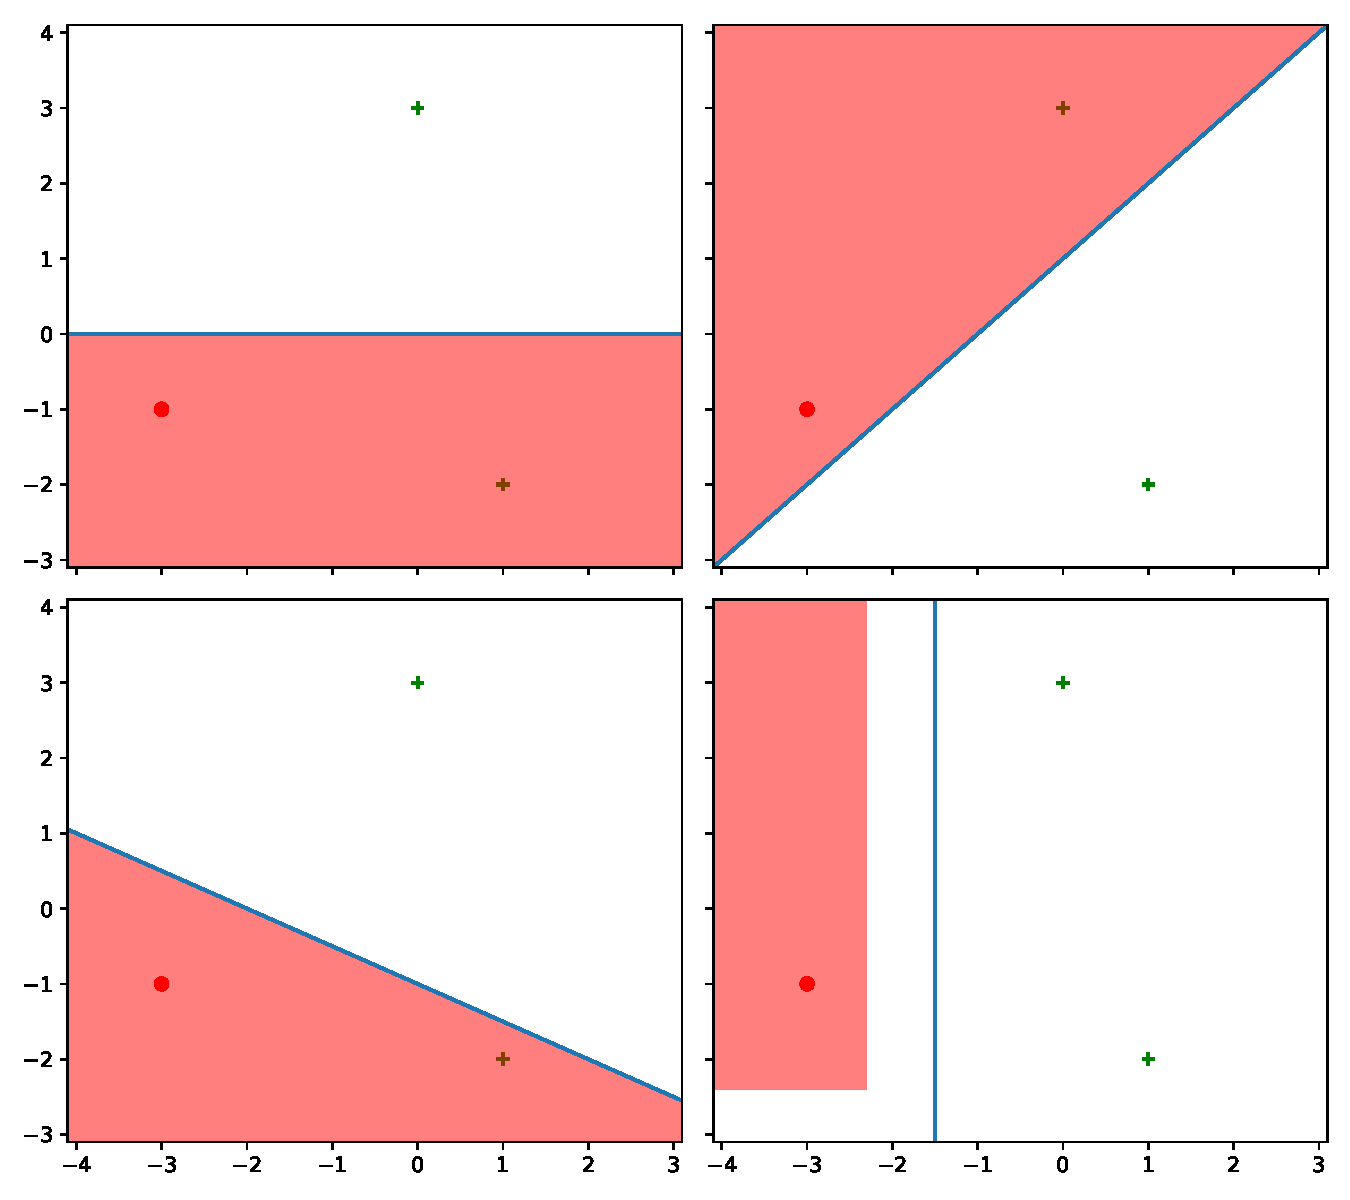
\includegraphics[width=0.4\textwidth]{separable_PLA.pdf}
    \caption{Perceptron's classifier visualised for each step.}
    % \label{fig:figure1}
  \end{figure}
\end{solution}

\begin{problem}[4]
  A dataset $S = \{(\mathbf{x}_1, y_1),\cdots,(\mathbf{x}_N, y_N)\} \subset \mathbb{R}^d \times \mathbb{R}$ is \emph{linearly separable} if there exists a perceptron that correctly classifies all data points in the set. In other words, there exists a hyperplane that separates positive data points and negative data points.

  In a 2D dataset, how many data points are in the smallest dataset that is not linearly separable, such that no three points are collinear? How about for a 3D dataset such that no four points are coplanar? Please limit your solution to a few lines - you should justify but not prove your answer.

  Finally, how does this generalize for an $N$-dimensional set, in which \textbf{no} $<$$N$-dimensional hyperplane contains a non-linearly-separable subset? For the $N$-dimensional case, you may state your answer without proof or justification.
\end{problem}
\begin{solution}
 For a 2D data set, the minimum number of data points to have a linearly inseparable set is four. For example, $\mathbf{x}=\{(0,1),(0,-1),(1,0),(-1,0)\}, y=\{+1,+1,-1,-1\}$ is a linearly inseparable set. In 3D, we would expect the five points to be the minimum dataset size to be linearly inseparable. We can generalise this as, if $N$ data points lies on one of the planes in $N$ dimensions, adding an additional point on one of these planes (for example) will still be separable. However, adding a second point on the same plane but on the opposite side of the origin will result in an inseparable set. 

 As such, we can say that, for an $N$ dimensional set, $N+2$ data points are the minimum required to have a set that is not linearly separable.
\end{solution}

\begin{problem}[2]
  Run the visualization code in the Jupyter notebook section corresponding to question C (report your plots). Assume a dataset is \emph{not} linearly separable. Will the Perceptron Learning Algorithm ever converge? Why or why not?
\end{problem}
\begin{solution}
  \begin{figure}[H]
    \centering
    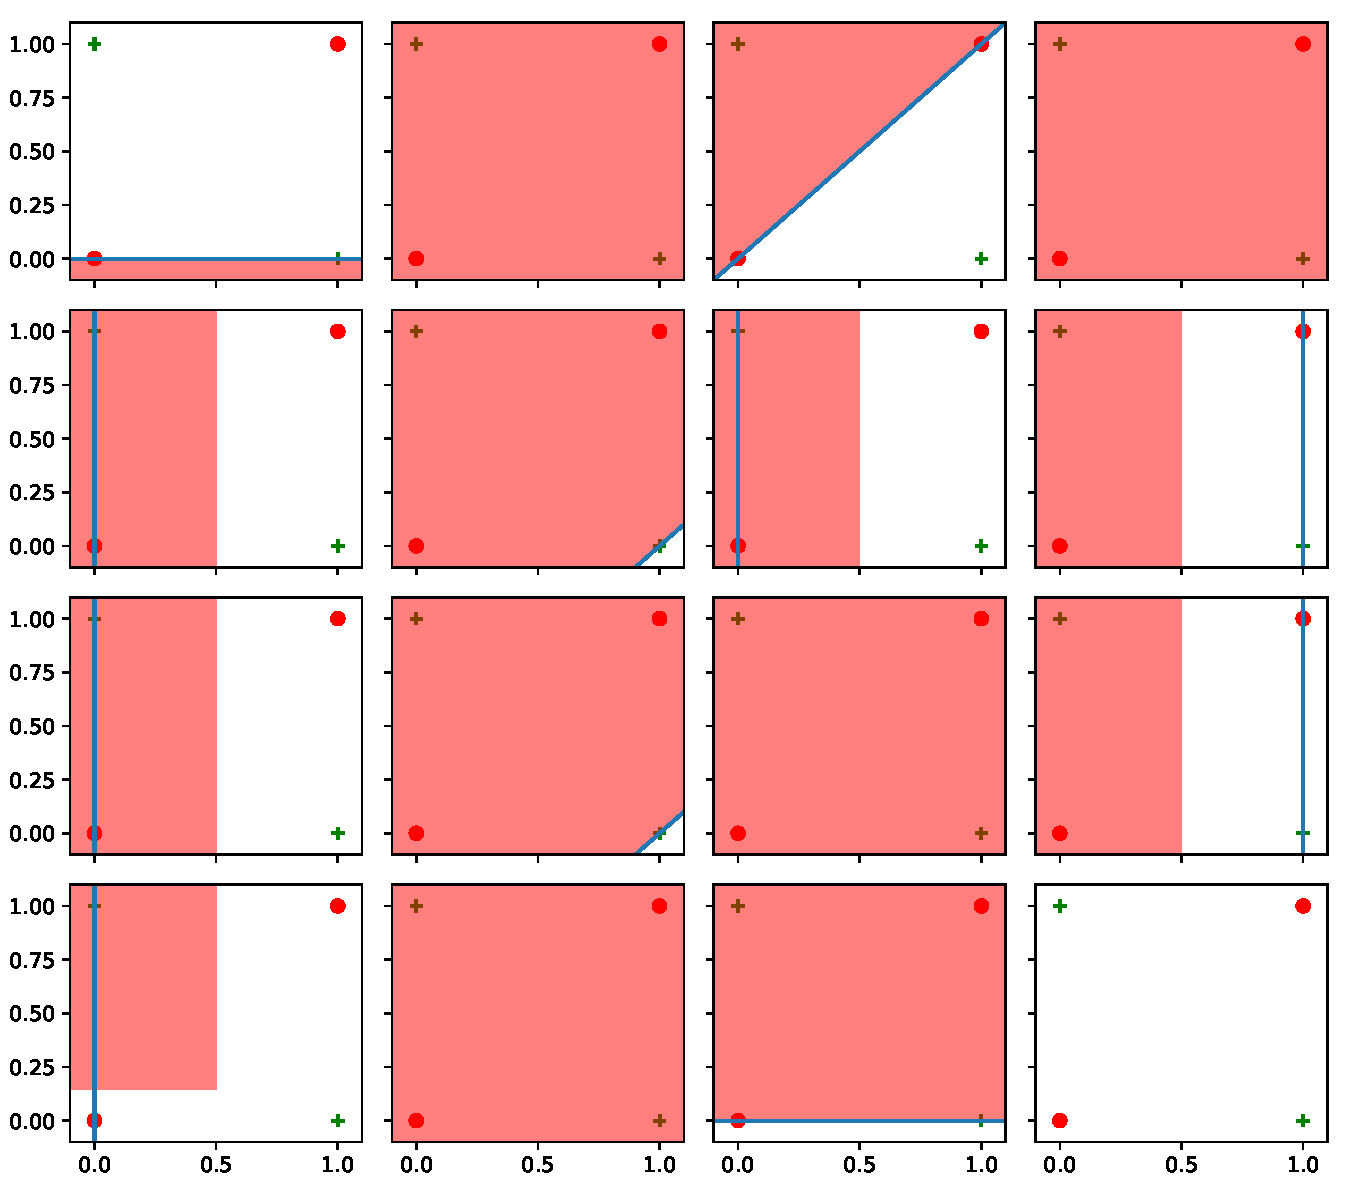
\includegraphics[width=0.4\textwidth]{unseparable_PLA.pdf}
    \caption{Perceptron's classifier visualised for each step for a linearly inseparable case.}
    % \label{fig:figure1}
  \end{figure}

  As shown above, if the dataset is not linearly separable, the PLA algorithm will never converge. This is because our stop condition is that all the variables are correctly classified. For such a data set, this will never be possible. As such, we just oscilate between different perceptrons.
\end{solution}

\end{document}